\section{Primary Challenges}

    \paragraph{}
    In this section, we will highlight the challenges associated with the sustainability of \gls{eh} batteryless \gls{mems} and \gls{iot} devices.

    \subsection{Dynamic Power Management}

        \paragraph{}
        \gls{dpm} is crucial in the realm of ultra-low power IoT devices, focusing on optimizing device performance to align with workload demands, thereby reducing unnecessary power usage and enhancing energy efficiency. This strategy is increasingly important as the adoption of mobile and battery-dependent IoT devices grows, alongside the need for energy-saving operations in data centers and cloud computing. Efficient DPM practices\cite{powerMngtIoT} are key to meeting these challenges, emphasizing the significance of energy management in advancing the sustainability and effectiveness of IoT technologies.

        \paragraph{}
        The challenge of \gls{dpm} lies in developing algorithms and techniques that can dynamically adjust the power states of computing devices in response to changing workload demands, resource availability, and system conditions. Several factors contribute to the complexity of \gls{dpm}, including heterogeneous workloads, real-time constraints, and uncertain workload patterns\cite{10387280}.

        \paragraph{}
        Efficient \gls{dpm} strategies play a crucial role in improving energy efficiency, extending battery life, reducing operating costs, and minimizing environmental impact in computing systems. However, existing approaches to \gls{dpm} often suffer from limitations such as overhead and complexity, sensitivity to workload variability, and trade-offs between energy and performance.

        \paragraph{}
        Future research directions in \gls{dpm} include:
        \begin{itemize}
            \item The development of \gls{adaptivealg} (e.g.: \gls{rehash}),
            \item The \gls{selflearningalg},
            \item Integration of \gls{ml} \cite{SABOVIC2023100736}, and
            \item Exploration of novel hardware architectures.
        \end{itemize}

        \paragraph{}
        Addressing the challenge of \gls{dpm} requires interdisciplinary research efforts spanning computer science, electrical engineering, and materials science, with the potential to drive innovation and reshape the future of computing technology.
        

    \subsection{Low-Power Hardware Design}

        \paragraph{}
        In the realm of batteryless systems, \gls{lphd} plays a pivotal role in enabling energy-efficient operation without reliance on traditional power sources like batteries. This approach focuses on crafting hardware components, such as processors, memory modules, and sensors, that consume minimal power while delivering optimal performance. This is crucial for extending the lifespan and enhancing the efficiency of batteryless \gls{iot} devices\cite{ultraLowPowerIntegratedCircuitDesign}.

        \paragraph{}
        \gls{lphd} in batteryless systems entails the development of components capable of operating efficiently in energy-constrained environments. This involves minimizing the average power consumption during operation and standby modes, as well as ensuring compatibility with \gls{eh} mechanisms to utilize ambient energy sources effectively.

        \paragraph{}
        Despite advancements, \gls{lphd} in batteryless systems presents several challenges. One of the primary hurdles is achieving a balance between power efficiency and performance. Ensuring high performance while operating within strict power constraints necessitates innovative design approaches and meticulous optimization.

        \paragraph{}
        The complexity of \gls{lphd} for batteryless systems stems from various factors:
        \begin{itemize}
            \item \textbf{Energy Constraints}: Devices, especially those reliant on battery or ambient energy, have limited power resources. This necessitates hardware that can operate efficiently under such constraints.
            \item \textbf{Technological Limitations}: Existing hardware components are often designed for performance, with less emphasis on energy efficiency. Redesigning them for low power consumption without sacrificing performance is challenging.
            \item \textbf{Integration Issues}: Combining low-power components with traditional energy sources and ensuring they work seamlessly with other parts of the system can be complex.
            \item \textbf{Heat Generation}: High-power consumption leads to heat generation, which can damage components and affect device reliability and lifespan.
        \end{itemize}

        \paragraph{}
        To address the challenges of \gls{lphd} in batteryless systems, researchers and engineers have developed several strategies:
        \begin{itemize}
            \item \textbf{Ultra-Low-Power Components}: Development of components that utilize minimal energy for operation. This includes low-power processors, memory, and sensors.
            \item \textbf{Energy-Efficient Architectures}: Designing system architectures that minimize energy waste, including power gating and energy-efficient communication protocols.
            \item \textbf{Adaptive Power Management}: Implementing dynamic power management techniques that adjust the energy consumption based on workload, thereby optimizing the power use in real-time.
            \item \textbf{Use of Advanced Materials}: Exploring new materials and manufacturing techniques that can reduce energy consumption and remove toxic component\cite{ecofriendlyManufacturingiot}, such as using silicon on insulator (SOI) technology or carbon nanotubes.
        \end{itemize}

        \paragraph{}
        Despite progress, \gls{lphd} in batteryless systems still faces limitations:
        \begin{itemize}
            \item \textbf{Performance Trade-offs}: Achieving ultra-low power consumption often requires sacrificing some level of performance, which may not be acceptable for all applications.
            \item \textbf{Complexity and Cost}: Designing and manufacturing low-power hardware components can be more complex and costly than traditional components, potentially limiting their adoption.
            \item \textbf{Technological Barriers}: There are physical and technological limits to how much power efficiency can be improved, especially with current materials and technologies.
            \item \textbf{Compatibility and Integration Challenges}: Ensuring that low-power components integrate seamlessly with existing systems and technologies without compromising functionality can be difficult.
        \end{itemize}

        \paragraph{}
        \gls{lphd} is a multifaceted challenge with significant implications for the future of sustainable and energy-efficient electronics. While the responses to this challenge have been innovative and impactful, they come with inherent limitations that require ongoing research and development. Overcoming these limitations necessitates a holistic approach, incorporating advances in materials science, electrical engineering, and computer science to pave the way for the next generation of low-power devices.



    \subsection{Energy-Aware Software Design}

        \paragraph{}
        \gls{easd} is a critical aspect of modern computing, focusing on the development of software systems and applications that prioritize energy efficiency alongside performance and functionality. This approach aims to minimize energy consumption during software execution, thereby extending battery life, reducing energy costs, and mitigating environmental impact.

        \paragraph{}
        This encompasses the creation of algorithms, programming methodologies, and software architectures that optimize energy usage limit the sacrificing performance or user experience. It involves identifying energy-intensive tasks, optimizing resource utilization, and leveraging energy-saving techniques to maximize efficiency across various computing platforms\cite{basedArticle}, \cite{protean}.

        \paragraph{}
        Despite its importance, energy-aware software design poses several challenges. One of the primary obstacles is achieving a balance between energy efficiency and performance. Ensuring that software operates with minimal energy consumption while meeting performance requirements requires careful consideration of algorithmic complexity, resource utilization, and system dynamics\cite{9803046}.

        \paragraph{}
        The complexity of energy-aware software design arises from various factors:
        \begin{itemize}
            \item Diverse application domains: Software applications span a wide range of domains, each with unique energy requirements and constraints, making it challenging to develop generic energy-saving strategies.
            \item Heterogeneous hardware platforms: Software must run on diverse hardware architectures, including mobile devices, embedded systems, and cloud servers, each with different power characteristics and optimization opportunities.
            \item Dynamic workload patterns: Workload characteristics may vary dynamically, necessitating adaptive software designs capable of adjusting energy usage in real-time based on workload demands and system conditions.
        \end{itemize}

        \paragraph{}
        To address the challenges of energy-aware software design, researchers and practitioners have developed several strategies:
        \begin{itemize}
            \item Energy-efficient algorithms: Designing algorithms optimized for low energy consumption without compromising computational performance or accuracy.
            \item \gls{energyaware} programming models: Developing programming models and frameworks that abstract hardware details and provide \gls{poweraware} abstractions to application developers.
            \item Dynamic energy management techniques: Implementing runtime systems and middleware that monitor system energy usage and dynamically adjust software behavior to optimize energy efficiency.
        \end{itemize}

        \paragraph{}
        Despite advancements, energy-aware software design faces limitations:
        \begin{itemize}
            \item Trade-offs between energy and performance: Optimizing for energy efficiency may result in performance degradation or increased execution time, impacting user experience and application responsiveness\cite{EHandEE}.
            \item Complexity and overhead: Implementing energy-aware techniques may introduce additional complexity and computational overhead, potentially negating energy savings achieved by the software.
            \item Compatibility and portability: Energy-aware software designs may not always be compatible with existing systems or easily portable across different hardware platforms, hindering adoption and interoperability\cite{basedArticle}.
        \end{itemize}
        
        \paragraph{}
        The energy-aware software design is essential for building sustainable computing systems and applications. Overcoming the challenges and limitations through continued research, innovation, and interdisciplinary collaboration is crucial for realizing the full potential of energy-efficient software design and driving advancements in computing technology.



    \subsection{Energy Harvesting Integration}
    
        \paragraph{}
        \gls{eh} integration is a vital aspect of modern electronics, focusing on the seamless incorporation of \gls{eh} mechanisms into electronic systems to enable self-powered operation. This approach aims to utilize ambient energy sources, such as solar, kinetic, or thermal energy, to generate electricity for powering electronic devices and systems without the need for external power sources.

        \paragraph{}
        This involves the design and implementation of electronic systems and components capable of efficiently harvesting, storing, and managing energy from ambient sources. It encompasses the integration of \gls{eh} modules, power management circuits, and energy storage elements into electronic devices, enabling them to operate autonomously and sustainably in various environments\cite{EHandEE}.

        \paragraph{}
        Despite its potential benefits, \gls{eh} integration presents several challenges. One of the primary obstacles is maximizing energy extraction efficiency while ensuring compatibility with the target application's power requirements. Achieving optimal \gls{eh} performance across different environmental conditions and device configurations requires careful system design and optimization.

        \paragraph{}
        The complexity of \gls{eh} integration arises from various factors:
        \begin{itemize}
            \item Variability of ambient energy sources: Ambient energy sources, such as solar radiation or mechanical vibrations, exhibit variability in intensity, duration, and availability, posing challenges for consistent \gls{eh}.
            \item Energy storage and management: Efficiently storing and managing harvested energy requires sophisticated power management techniques and energy storage technologies capable of handling fluctuating energy inputs and varying power demands.
            \item Integration with existing systems: Retrofitting \gls{eh} capabilities into existing electronic systems or integrating them into new designs without compromising functionality or performance presents integration challenges.
        \end{itemize}

        \begin{figure}[htbp]
            \centering
            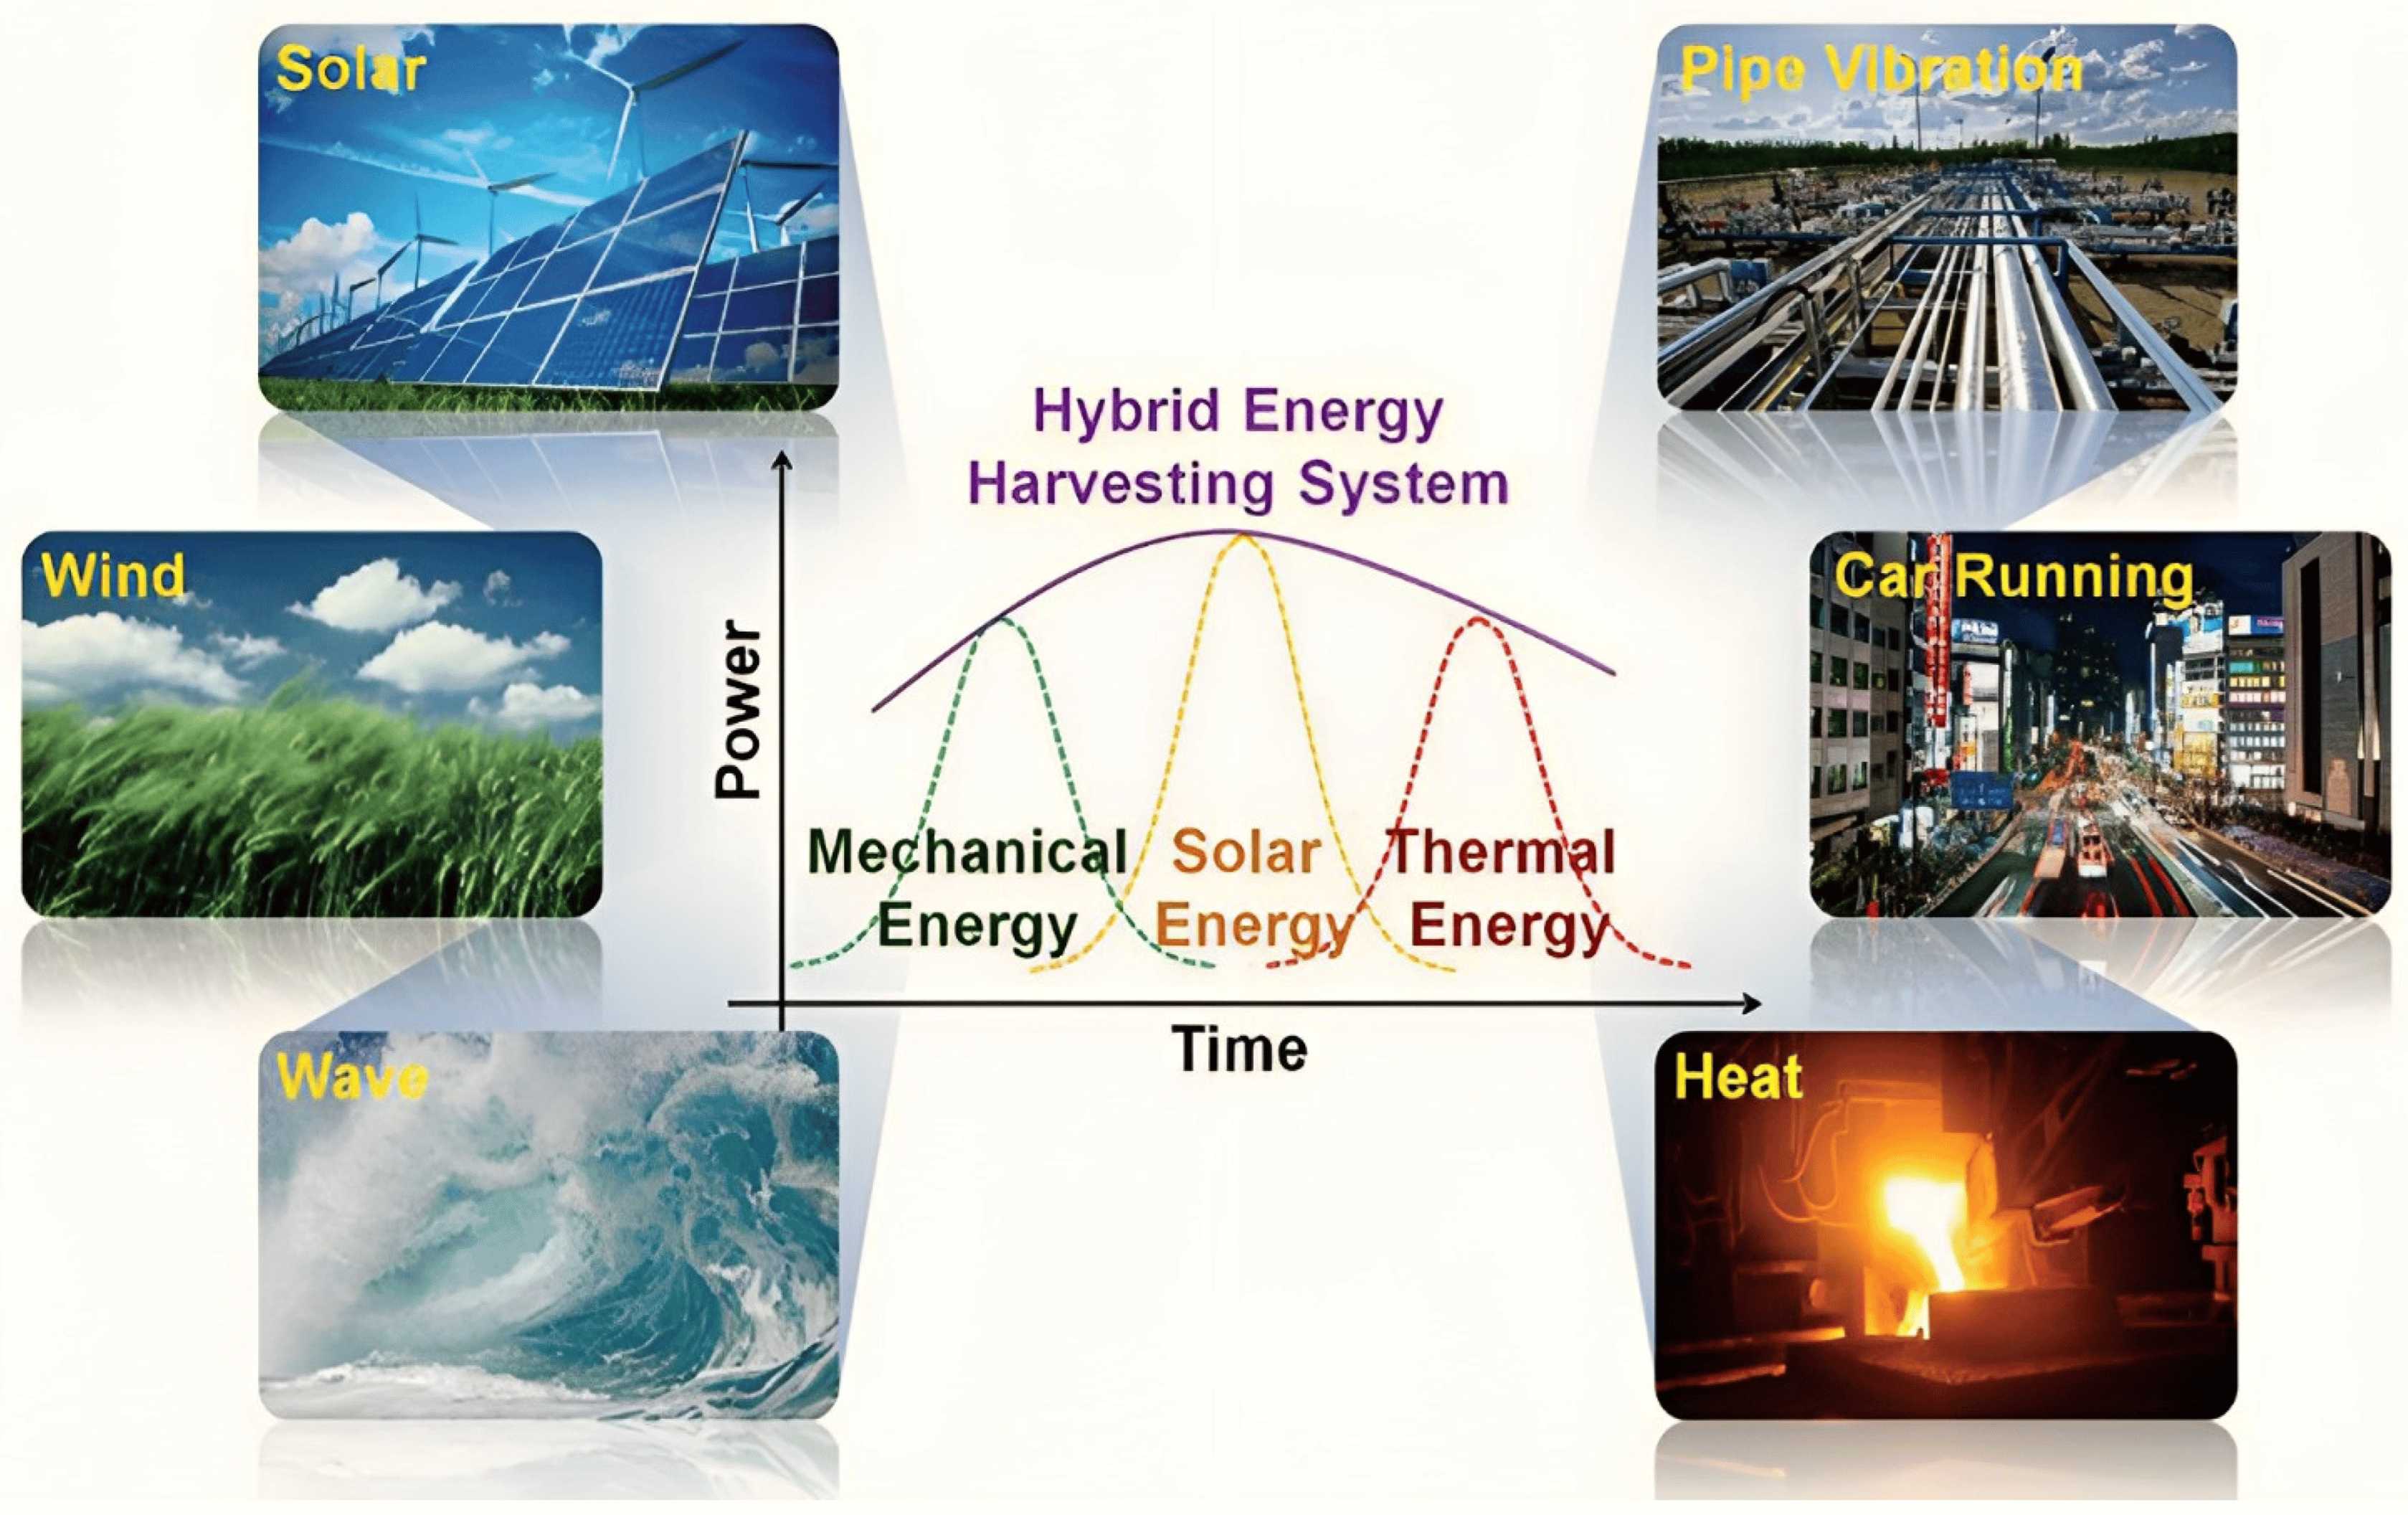
\includegraphics[width=0.9\textwidth]{img/003_EnergyHarvestingDevices.png}
            \caption{Diagram of a hybrid energy harvesting that uses both artificial and natural energies. \cite{jlpea13040062}, Page 3.}
            \label{fig:EnergyHarvestingDevices}
        \end{figure}

        \paragraph{}
        To address the challenges of \gls{eh} integration, researchers and engineers have developed several strategies:
        \begin{itemize}
            \item Adaptive \gls{eh} systems: Designing \gls{eh} systems equipped with adaptive algorithms and control mechanisms that optimize \gls{eh} performance based on environmental conditions and power requirements.
            \item Hybrid \gls{eh} approaches (figure \ref{fig:EnergyHarvestingDevices}, \cite{jlpea13040062}): Combining multiple \gls{eh} techniques, such as solar, kinetic, and thermal harvesting, to increase energy diversity and reliability and mitigate the limitations of individual harvesting methods.
            \item System-level optimization: Optimizing the overall system architecture, including \gls{eh} modules, power management circuits, and energy storage components, to maximize energy efficiency and system robustness.
        \end{itemize}

        \paragraph{}
        In summary, \gls{eh} integration holds great promise for enabling self-powered electronic systems and reducing reliance on external power sources. Overcoming the challenges and limitations through continued research, innovation, and collaboration is essential for realizing the full potential of \gls{eh} integration and driving advancements in sustainable electronics.
        


    \subsection{Adapting to Intermittent Energy Supply}

    \paragraph{}
    In the context of \gls{iot}, batteryless, and ultra-low power technologies, \gls{ies} refers to the challenge of ensuring continuous operation under conditions of fluctuating energy availability. This is particularly relevant for IoT devices deployed in remote or energy-constrained environments, where energy sources such as solar, ambient RF, or thermal gradients are subject to variability. The key is to harness these intermittent energy sources efficiently to power devices that require minimal energy for operation\cite{gameboyBatteryless}, \cite{basedArticle}.

    \paragraph{}
    The adaptation involves developing energy harvesting technologies and ultra-low power circuits that can operate in environments with highly variable energy inputs. Unlike traditional systems that rely on consistent power sources, IoT and ultra-low power devices must be designed to function effectively even with sporadic energy availability, leveraging the smallest amounts of energy for maximum utility\cite{EHandEE}.

    \paragraph{}
    The primary challenge in this domain is designing systems that are resilient to energy fluctuations, ensuring that IoT devices can maintain functionality without constant power supply. This includes optimizing energy storage, utilizing innovative batteryless technologies, and implementing power management strategies that adjust device operations based on available energy.

    \paragraph{}
    The complexity of adapting to \gls{ies} in IoT and ultra-low power systems involves several factors:
    \begin{itemize}
        \item Energy harvesting efficiency: Developing technologies capable of converting ambient energy sources into usable power with high efficiency, even under varying environmental conditions.
        \item Power management: Designing advanced power management circuits that minimize energy consumption and dynamically adjust device operations based on the current energy availability.
        \item Batteryless and energy storage solutions: Exploring innovative batteryless technologies and ultra-low power energy storage solutions that can provide reliable power supply despite intermittent energy generation.
    \end{itemize}

    \paragraph{}
    To address these challenges, various strategies have been developed:
    \begin{itemize}
        \item Adaptive energy harvesting: Implementing adaptive energy harvesting techniques that can optimize energy conversion from available sources in real-time, ensuring maximum power extraction.
        \item Ultra-low power design: Designing IoT devices and components that operate with minimal power consumption, extending operational life and reducing the need for frequent energy replenishment.
        \item Intelligent power management: Utilizing smart power management algorithms that dynamically balance energy harvesting, storage, and consumption to maintain continuous device operation.
    \end{itemize}

    \paragraph{}
    Despite advancements, adapting to \gls{ies} in the context of IoT, batteryless, and ultra-low power technologies poses several limitations:
    \begin{itemize}
        \item Operational constraints under low energy conditions: Ensuring reliable device functionality when energy availability is minimal remains a challenge.
        \item Energy storage and conversion efficiency: Improving the efficiency of energy storage and conversion mechanisms is critical for maximizing the utility of harvested energy.
        \item Integration and scalability: Integrating these technologies into a wide range of devices and applications, and scaling them to meet diverse operational requirements, presents ongoing challenges.
    \end{itemize}
    
    \paragraph{}
    Addressing the challenges of \gls{ies} in IoT, batteryless, and ultra-low power contexts requires innovative approaches that combine technological advancements, design optimization, and strategic power management. Overcoming these challenges is crucial for expanding the deployment of IoT devices in energy-constrained environments, paving the way for a more connected, efficient, and sustainable world.


    
    \subsection{Sensor Optimization}
    
        \paragraph{}
        Sensor optimization is a critical aspect of sensor design and deployment, focusing on enhancing the performance, efficiency, and reliability of sensors in various applications. This involves optimizing sensor parameters, configurations, and algorithms to achieve accurate and timely data acquisition while minimizing energy consumption and resource utilization.

        \paragraph{}
        Sensor optimization encompasses a range of techniques and strategies aimed at improving the effectiveness and efficiency of sensors. This includes optimizing sensor placement, calibration, sampling rates, and signal processing algorithms to maximize the quality and utility of sensor data while minimizing power consumption, latency, and cost\cite{ultraLowPowerIntegratedCircuitDesign}, \cite{EHandEE}.

        \paragraph{}
        The primary challenge of sensor optimization lies in achieving a balance between sensor performance and resource constraints. Designing sensors that deliver accurate and timely data while operating within limited power, memory, and processing resources requires careful optimization and trade-offs.

        \paragraph{}
        The complexity of sensor optimization arises from various factors:
        \begin{itemize}
            \item Resource constraints: Sensors deployed in resource-constrained environments, such as \gls{iot} devices or wireless sensor networks, must operate within strict limitations on power consumption, memory usage, and processing capabilities.
            \item Environmental variability: Environmental factors such as temperature, humidity, and interference can affect sensor performance and reliability, necessitating robust optimization techniques to mitigate their impact.
            \item Application-specific requirements: Sensors deployed in different applications, such as environmental monitoring, healthcare, or industrial automation, have unique requirements and constraints that must be considered during optimization.
        \end{itemize}

        \paragraph{}
        To address the challenges of sensor optimization, various strategies have been developed:
        \begin{itemize}
            \item Energy-efficient sensor design: Designing sensors with low-power components, optimized circuitry, and energy-efficient communication protocols to minimize power consumption and extend battery life.
            \item Adaptive sensing algorithms: Developing adaptive sensing algorithms that dynamically adjust sensor parameters and sampling rates based on environmental conditions, user requirements, and energy availability to optimize performance and efficiency.
            \item Distributed sensor networks: Deploying distributed sensor networks with decentralized processing and collaborative sensing capabilities to distribute computation and reduce energy consumption.
        \end{itemize}

        \paragraph{}
        Despite advancements, sensor optimization poses several limitations:
        \begin{itemize}
            \item Trade-offs between performance and resource consumption: Optimizing sensor performance may require increased power consumption, memory usage, or processing resources, leading to trade-offs that impact overall system efficiency and scalability.
            \item Sensing accuracy and reliability: Optimized sensor configurations and algorithms may sacrifice accuracy or reliability under certain conditions, affecting the quality and usefulness of sensor data.
            \item Complexity and implementation challenges: Implementing sophisticated optimization techniques and algorithms may introduce complexity and overhead, requiring specialized expertise and resources for design, development, and deployment.
        \end{itemize}

        \paragraph{}
       The sensor optimization is essential for maximizing the effectiveness and efficiency of sensor systems in various applications. Overcoming the challenges and limitations through continued research, innovation, and collaboration is crucial for realizing the full potential of sensor technology and enabling transformative applications in fields such as \gls{iot}, healthcare, environmental monitoring, and beyond.
        

    \paragraph{}
    In conclusion, addressing the sustainability of \gls{eh} batteryless \gls{iot} devices requires a multifaceted approach that tackles the challenges of \gls{dpm}, low-power hardware and software design, \gls{eh} integration, \gls{ies}, and sensor optimization. Overcoming these challenges necessitates ongoing research, innovation, and interdisciplinary collaboration to develop solutions that are not only energy-efficient but also practical, reliable, and scalable.